
\chapter{四足機器人}
\begin{figure}[hbt!]
\begin{center}
\label{四足機器人步驟圖}
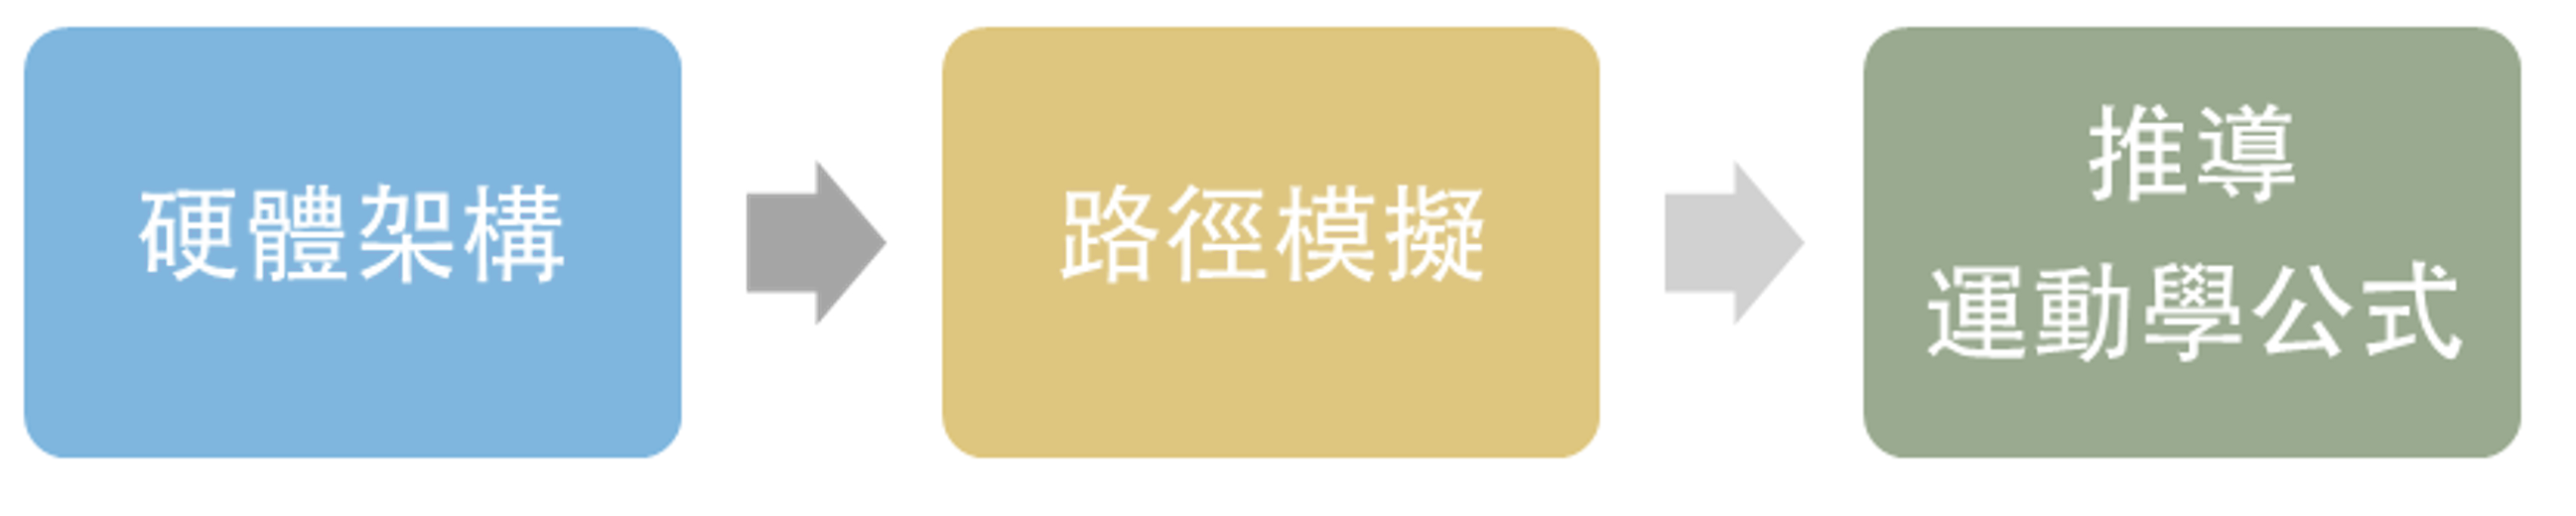
\includegraphics[width=14cm]{四足機器人步驟圖}
\caption{\Large 運動學推導流程}
\end{center}
\end{figure}
本章節將對四足機器人進行介紹並利用虛擬環境進行模擬運動情況,透過仿真環境找出四足機器人的最大反力並利用運動學公式計算行走姿態路徑。\\

%--------------------應用範圍反作用--------------------%
\section{應用範圍及作用}


四足機器人為一種模仿動物運動的機器人,分別由四組步行機構及本體組成,利用電子元件驅動機械臂進行運動,可用以替代人力執行任務,同時為人們帶來許多樂趣及益處,可大致上分為以下幾種類型:\\

\begin{enumerate}
\item 軍事:四足機器人有良好的機械性能,搭配著電子控制系統,可以輕鬆在各地形中運輸物品及人員,感測器的回饋、馬達的行程及出力大小,在戰場中穿梭及運輸補給品,或是在搜救行動當作先鋒隊,都不是問題,可以減低人員受傷的危險。\
\item 工業:替代傳統人力,保持高效運作,減少作業人員在高風險環境中造成職業傷害,也減少工業中的資源浪費。\
\item 民生:可以執行各種控制指令,可以體驗仿生機器人的操作特性和樂趣,也可以幫助幫運重物,也能依照需求進行各式改裝及編程,讓四足機器人可以達到所需的功能。\
\end{enumerate}
\newpage

隨著電腦的普及,各式各樣的編程軟體如雨後春筍般誕生,計算機語言也更好上手,讓更多使用者可以輕而易舉的使用,也有許多人在網路公開分享開源的程式及經驗可以參考及學習,配合現在AI的發展,四足機器人應用範圍越加的廣泛,正因為如此我們才以四足機器人為主題,研究由誕生至成品將會有哪些步驟及考量。\\

%----------------步行結構運動學模型介紹---------------%
\section{連桿閉環機構}
在步行結構設計之初,通常透過模仿生物,來創造不同的機械模型,不同型態的機械模型都有其各自特性,對於連接機構的運動控制,一般來說,腿部的機械結構不能過於複雜,過多的機械零件需要較精細的控制元件及設計,對於控制運動軌跡及製作成本來說較不益,以下為Goegebra所繪製連桿機構講述:\\

\begin{figure}[htbp]
  \begin{minipage}[t]{0.5\linewidth}
    \centering
    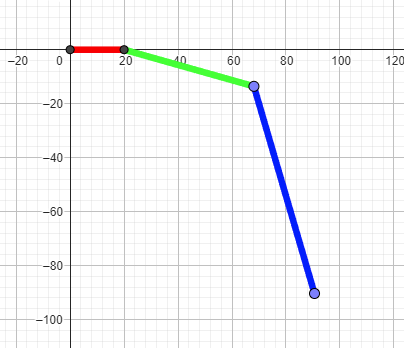
\includegraphics[height=6cm,width=6cm]{三連桿閉環機構}
    \caption{三連桿閉環機構}
    \label{三連桿閉環機構}
  \end{minipage}
  \hfill
  \begin{minipage}[t]{0.4\linewidth}
    \centering
    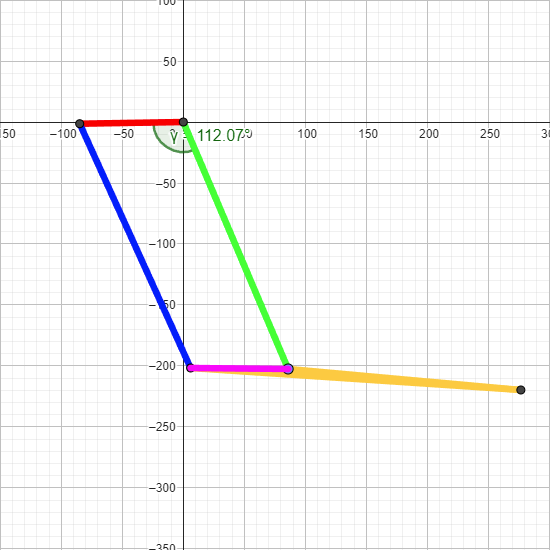
\includegraphics[height=6cm,width=6cm]{步行機構ggb}
    \caption{四連桿閉環機構}
    \label{步行機構ggb}
  \end{minipage}
\end{figure}

\begin{enumerate}
\item 三連桿閉環機構:\\

此三連桿閉環機構(圖 \ref{三連桿閉環機構})為三個連桿及三顆馬達組成,此機構以一個關節連接本體,結構較為緊湊、簡單,通過三連桿關節的旋轉角度控制整體機構做動及末端點位置,具有靈活性高、反應快速、定位精度高等優點。\

\item 四連桿閉環機構:\\

此四連桿閉環機構(圖 \ref{步行機構ggb})為四個連桿及兩顆馬達組成,組成一個不規則四邊形,兩個馬達分別驅動Leg1-5(綠)及Leg2(紅)桿件搖擺,互相搭配後讓連桿有大幅度的運動,此機構較為複雜,需要較精細的控制以實現穩定的運動,有著能承受較大負載的優勢,對於運動穩定性也有著良好的表現,為此專題步行裝置所參考的機構。\\

\end{enumerate}

%----------------硬體架構---------------%
\section{硬體架構}
\begin{figure}[hbtp]
\begin{center}
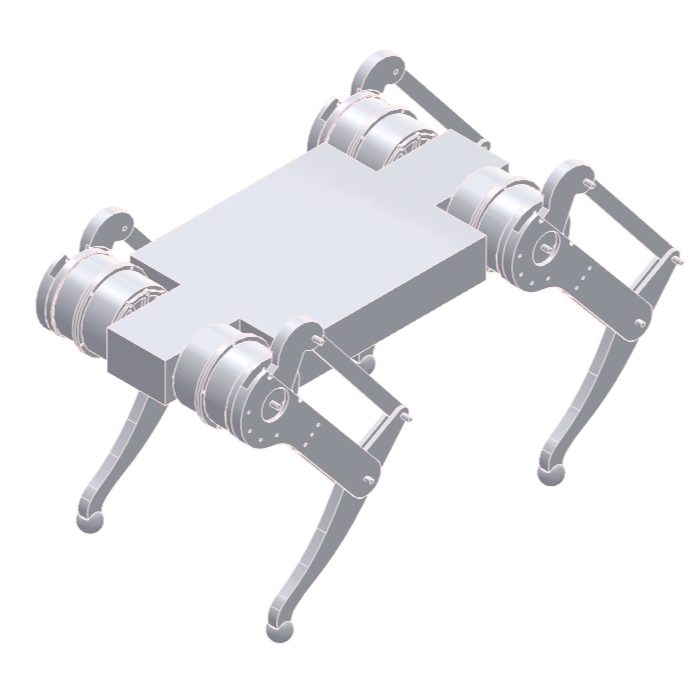
\includegraphics[width=9cm]{四足機器狗}
\caption{\Large 四足機器人}\label{四足機器狗}
\end{center}
\end{figure}

(圖 \ref{四足機器狗})所示為本次專題研究的有限元素法分析對象,四足機器人的的站立姿態,由四組步行機構及一個本體和馬達及連接板組成硬體結構,因為本專題研究的機器人需要有高負重及高穩定性,所以使用上述所講的四連桿閉環機構。\

\newpage

\begin{figure}[hbt!]
\begin{center}
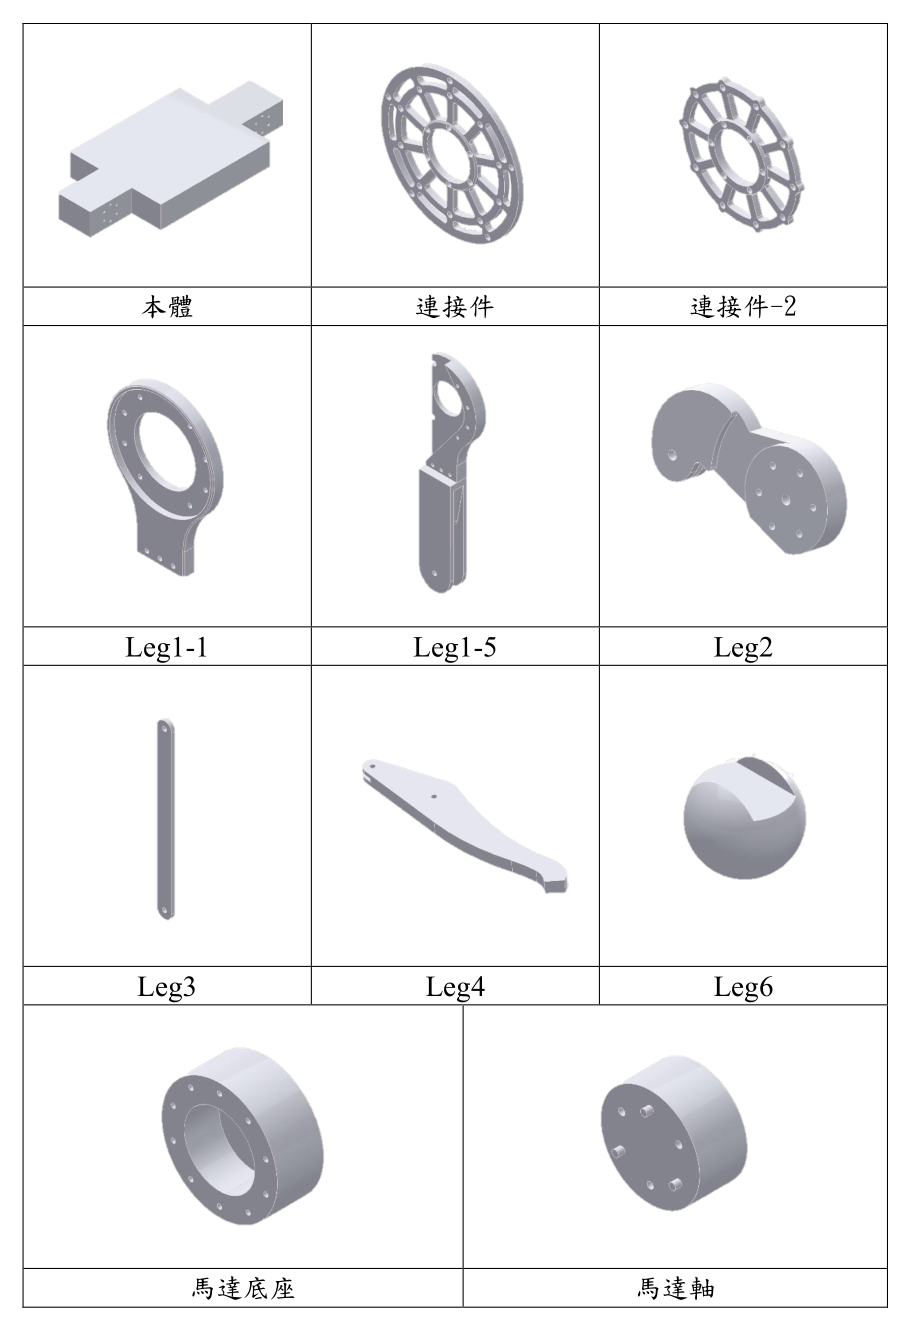
\includegraphics[width=15cm]{零件表}
\caption{\Large 零件表}\label{零件表}
\end{center}
\end{figure}

\newpage

%----------------運動軌跡---------------%

\section{運動軌跡}
Leg1-5的長度為半徑建立圓形,且給定數值滑桿(一)控制Leg1-5末端點並限制其角度;Leg2的長度為半徑生成Leg2末端點,且給定數值滑桿(2)控制Leg2末端點並限制其角度。\\

將兩點設定為搖擺運動,以Leg2末端點為圓心繪製半徑長為Leg3的圓形,再於Leg1-5末端點以L3’為半徑畫圓,即可找出兩圓交點並連接,再用Leg1-5末端點及Leg3末端點為圓心,兩點和目標點距離為半徑畫圓,兩圓交點部分即為目標點,由此可得模擬路徑範圍如下圖所示:\\
\begin{figure}[hbt!]
\begin{center}
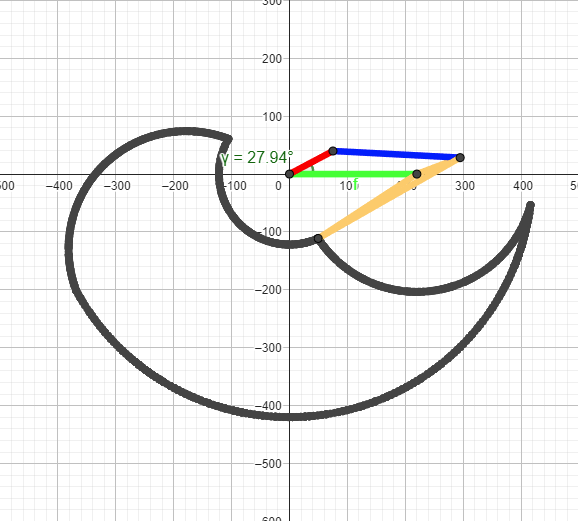
\includegraphics[width=14cm]{機械腿運動軌跡}
\caption{\Large Geogebra運動軌跡}\label{機械腿運動軌跡}
\end{center}
\end{figure}

\newpage

%-------------四連桿機構運動學模型---------------%
\section{四連桿機構運動學模型}

\begin{figure}[htbp]
  \begin{minipage}[t]{0.5\linewidth}
    \centering
    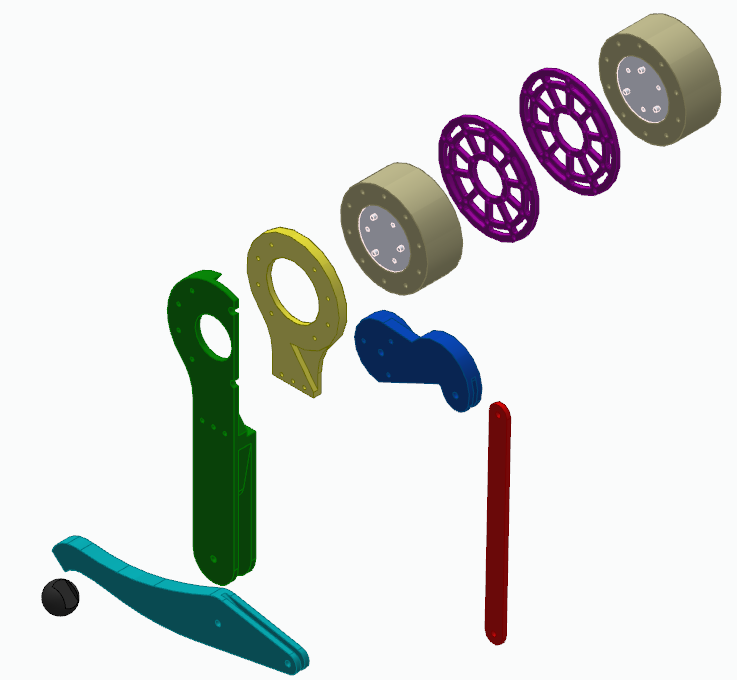
\includegraphics[height=6cm,width=6cm]{步行機構分解圖}
    \caption{步行機構分解圖}
    \label{步行機構分解圖}
  \end{minipage}
  \hfill
  \begin{minipage}[t]{0.4\linewidth}
    \centering
    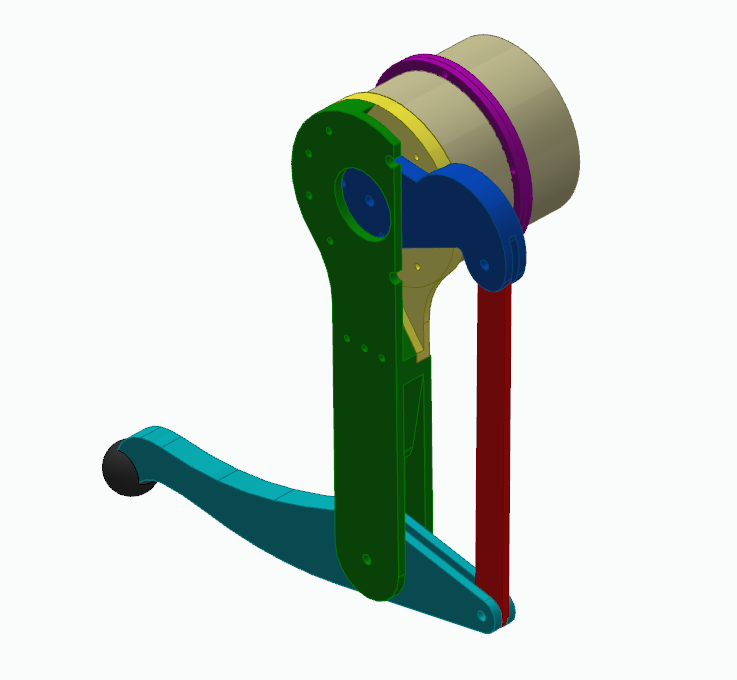
\includegraphics[height=6cm,width=6cm]{步行機構}
    \caption{步行機構}
    \label{步行機構}
  \end{minipage}
\end{figure}

\begin{figure}[htbp]
  \begin{minipage}[t]{0.5\linewidth}
    \centering
    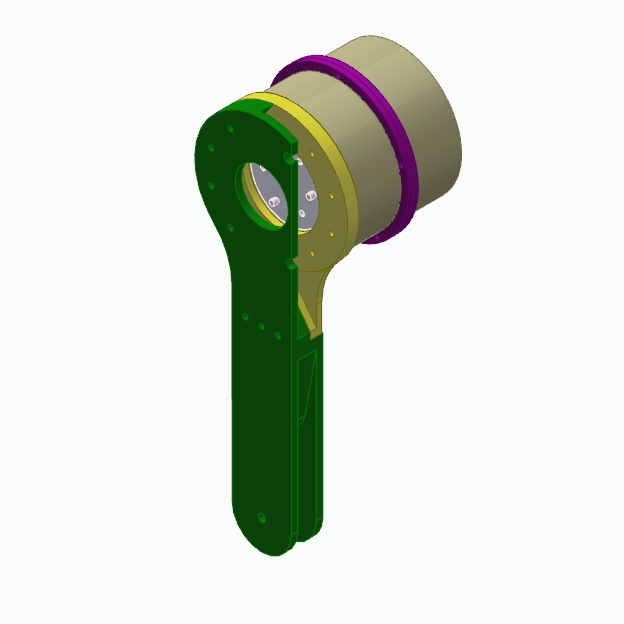
\includegraphics[height=6cm,width=6cm]{馬達(一)控制件}
    \caption{馬達(一)}
    \label{馬達(一)控制件}
  \end{minipage}
  \hfill
  \begin{minipage}[t]{0.4\linewidth}
    \centering
    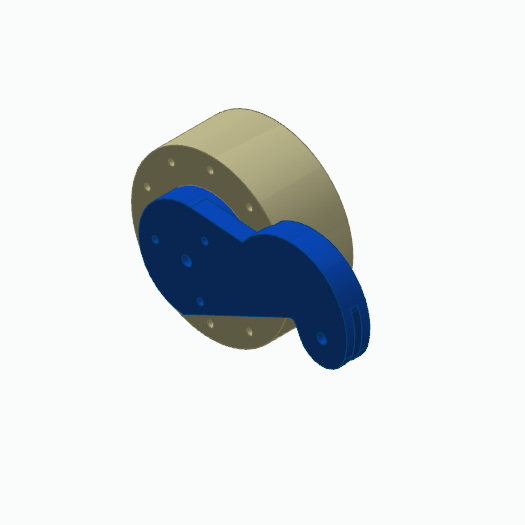
\includegraphics[height=6cm,width=6cm]{馬達(二)控制件}
    \caption{馬達(二)}
    \label{馬達(二)控制件}
  \end{minipage}
\end{figure}

A部分:由馬達(一)所控制的結構為零件Leg1-1(黃)和Leg1-5(綠);B部分:由馬達(二)所驅動的結構為零件Leg2(藍)。\\

連桿Leg3(紅)B部份所控制,被動對Leg4(青)施以推力及拉力,因此Leg4(青)中間受A部分連桿約束後將會控制Leg6(橡膠套)做動。\\

此順向運動學將對步行機構(圖 \ref{步行機構分解圖})至(圖 \ref{步行機構})進行計算馬達旋轉角,推導順逆向運動學,由於四組步行機構為相同模型,因此只要提出其中一組計算即可。\
\newpage

\subsection{順向運動學}

\begin{figure}[hbt!]
\begin{center}
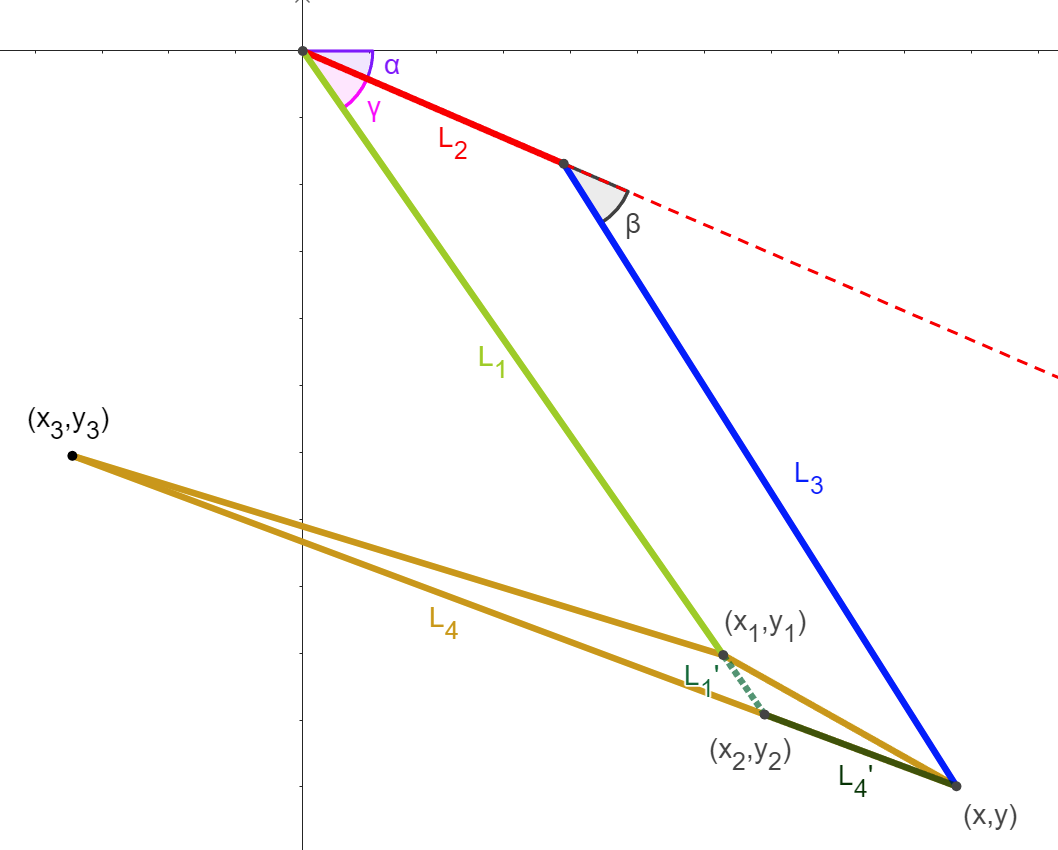
\includegraphics[width=11cm]{Forward kinematics formula}
\caption{\Large 順向運動學連桿圖}\label{Forward kinematics formula}
\end{center}
\end{figure}

可見A部分為二連桿機構組成,因此使用三角函數即可分別計算出末端點的相對座標位置,可以繪出連桿圖及列出算式如下:\\

($x$,$y$)座標
\[
\begin{aligned}
x&=L_{2}\cos \alpha +L_{3}\cos \left( \alpha +\beta \right)\\
y&=L_{2}\sin \alpha +L_{3}\sin \left( \alpha +\beta \right)\\
\end{aligned}
\]\\

B部份則為單支連桿組成,套入三角函數的計算方式如下:\\

\[
\begin{aligned}
x_{1}&=L_{1}\cos \left( \alpha +\gamma \right)\\
y_{1}&=L_{1}\sin \left( \alpha +\gamma \right)\\
\end{aligned}
\]\\

求出A部分($x$,$y$)座標連接到末端點($x_3$,$y_3$),再以內分點公式求出$L_1$延伸至$L_4$之交點:\

$L_4$:為($x_3$,$y_3$)至($x$,$y$)長度\

$L_4$':為($x_2$,$y_2$)至($x$,$y$)長度\\

\[
\begin{aligned}
x_{2}&= \frac{\left (L_{1} + L_{1}' \right) x_{1}}{L_{1}}\\
y_{2}&= \frac{\left (L_{1} + L_{1}' \right) y_{1}}{L_{1}}\\
\end{aligned}
\]\\

找出點($x$,$y$)及點($x_2$,$y_2$)用內分點公式求出末段點與地面交點:

\[
\begin{aligned}
x_{3}&= \frac{L_{4} x_{2} - \left (L_{4} - L_{4}' \right) x}{L_{4}'}\\
y_{3}&= \frac{L_{4} y_{2} - \left (L_{4} - L_{4}' \right) y}{L_{4}'}\\
\end{aligned}
\]\\

由此公式得出目標末端點相對至基座連結關節座標,以利於控制\\

\subsection{逆向運動學}
與順向運動學不同是,此種求解方法需要先定義末端位置和姿態,通過觀察機械系統的末端位置推導,計算出各關節的運動及整體姿態,通常以非線性方程組問題表示,其中每個方程都可代表著一個機械臂關節的末端位置及角度,因此需要使用數值方法去求解,本專題透過電腦計算,利用模擬求出座標點。\\

作用於機器人在空間中精準控制末端姿態,在機器臂控制、機器人視覺和機器人運動學等領域有著許多應用的地方。\
\newpage

下方表格為我們在GeoGebra取得的橢圓及直線足端路徑座標點及角度,可以利用查表找出步行機構足端到達該座標點所需的旋轉角度。我們將列出其中兩種軌跡,其餘路徑(圖 \ref{足端軌跡(不規則)})皆可製作成此種表格。\\

\begin{table}[htb!]
  \center
  \large
  \caption{\Large 足端橢圓運動軌跡}
  \setlength{\tabcolsep}{0.5cm}{
  \begin{tabular}{|c|c|c|c|c|c|c|}
    \hline 代號 & A & B & C & D & E & F \\
    \hline $x_3$ & 52.03 & 2.10 & -67.03 & -142.53 & -64.46 & 4.92  \\
    \hline $y_3$ & -217.45 & -219.07 & -226.33 & -252.41 & -291.39 & -297.92  \\
    \hline $\alpha$ & $31.90^\circ$ & $18.30^\circ$ & $3.88^\circ$ & $0.10^\circ$ & $18.42^\circ$ & $31.75^\circ$  \\
    \hline $\beta$ & $55.46^\circ$ & $54.19^\circ$ & $59.07^\circ$ & $76.24^\circ$ & $79.24^\circ$ & $79.07^\circ$  \\
    \hline $\gamma$ & $53.84^\circ$ & $52.54^\circ$ & $57.52^\circ$ & $74.89^\circ$ & $77.91^\circ$ & $77.74^\circ$ \\
    \hline 代號 & G & H & I & J & K & ~ \\
    \hline $x_3$ & 104.82 & 174.02 & 254.19 & 199.84 & 121.16 & ~\\
    \hline $y_3$ & -297.58 & -290.62 & -253.76 & -229.59 & -219.50 & ~\\
    \hline $\alpha$ & $53.50^\circ$ & $69.72^\circ$ & $88.44^\circ$ & $73.03^\circ$ & $51.61^\circ$ & ~\\
    \hline $\beta$ & $85.54^\circ$ & $94.88^\circ$ & $104.12^\circ$ & $81.39^\circ$ & $63.49^\circ$ & ~\\
    \hline $\gamma$ & $84.23^\circ$ & $93.57^\circ$ & $102.78^\circ$ & $80.07^\circ$ & $62.01^\circ$ & ~\\
    \hline
  \end{tabular}}
\end{table}

\begin{table}[htb!]
  \center
  \large
  \caption{\Large 足端直線運動軌跡}
  \setlength{\tabcolsep}{0.72cm}{
  \begin{tabular}{|c|c|c|c|c|c|}
    \hline 代號 & A & B & C & D & E \\
    \hline $x_3$ & -200 & -160 & -120 & -80 & -40 \\
    \hline $y_3$ & -300 & -300 & -300 & -300 & -300 \\
    \hline $\alpha$ & $10.03^\circ$ & $11^\circ$ & $13.75^\circ$ & $18.21^\circ$ & $24.07^\circ$  \\
    \hline $\beta$ & $104.75^\circ$ & $95.42^\circ$ & $88.49^\circ$ & $83.64^\circ$ & $80.76^\circ$  \\
    \hline $\gamma$ & $103.44^\circ$ & $94.11^\circ$ & $87.18^\circ$ & $82.33^\circ$ & $79.44^\circ$  \\
    \hline
    代號 & F & G & H & I & J \\
    \hline $x_3$ & 0 & 40 & 80 & 120 & 160 \\
    \hline $y_3$ & -300 & -300 & -300 & -300 & -300 \\
    \hline $\alpha$ & $31.18^\circ$ & $39.26^\circ$ & $48.07^\circ$ & $57.39^\circ$ & $67.15^\circ$  \\
    \hline $\beta$ & $79.8^\circ$ & $80.76^\circ$ & $83.64^\circ$ & $88.49^\circ$ & $95.42^\circ$  \\
    \hline $\gamma$ & $78.48^\circ$ & $79.44^\circ$ & $82.33^\circ$ & $87.18^\circ$ & $94.11^\circ$  \\
    \hline
  \end{tabular}}
\end{table}
\newpage

